\documentclass{standalone}
\usepackage{tikz, ifthen}
\usepackage{amsmath}

\begin{document}

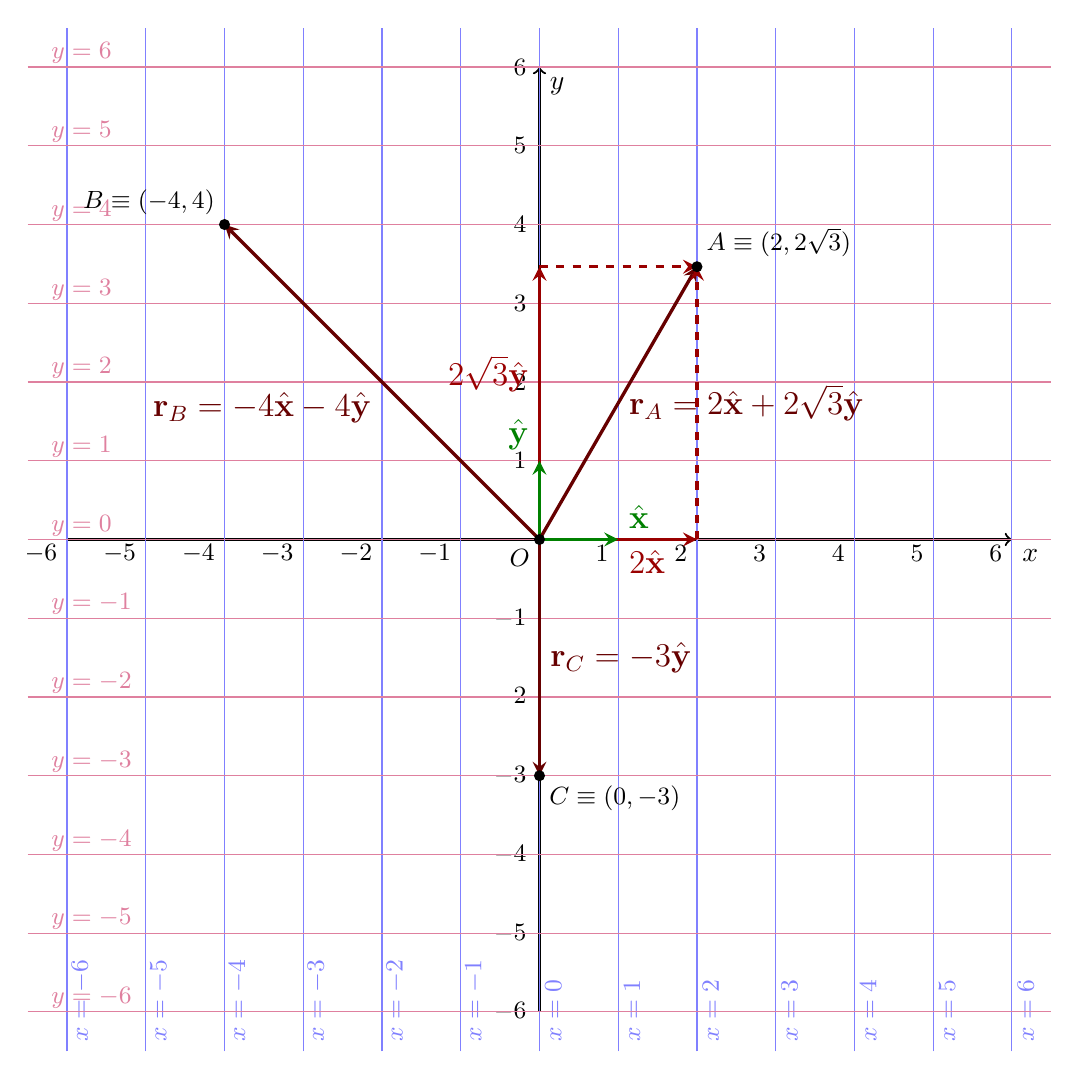
\begin{tikzpicture}
    
    % Center of the circle
    \def\xmin{-6}
    \def\xmax{6}
    \def\ymin{-6}
    \def\ymax{6}
    \def\dx{.5}
    \def\dy{.5}
    \def\xminb{\xmin-\dx}
    \def\xmaxb{\xmax+\dx}
    \def\yminb{\ymin-\dy}
    \def\ymaxb{\ymax+\dy}
    \def\xo{2}     % translation, x
    \def\yo{1.5}   % translation, y
    \def\xpmin{-6}
    \def\xpmax{ 6}
    \def\ypmin{-5.5}
    \def\ypmax{ 5.5}

    % Fill outside region
    \clip (\xminb, \yminb) rectangle (\xmaxb, \ymaxb);
    
    % Axes, x
    \draw[->, thick, black] (\xmin, 0) -- (\xmax, 0) node[below right] {$x$};
    \draw[->, thick, black] (0, \ymin) -- (0, \ymax) node[below right] {$y$};
    % Axis ticks
    \foreach \x in {\xmin,..., \xmax}{
        \ifthenelse{ \x = 0 }{}{\draw[black] (\x, -0.1) -- (\x, +0.1) node[below=8pt, left=0pt] {\small $\x$};}
    }
    \foreach \y in {\ymin,..., \ymax}{
        \ifthenelse{ \y = 0 }{}{\draw[black] (-0.1, \y) -- (0.1, \y) node[left=4pt] {\small $\y$};}
    }
    
    % Axis ticks
    \foreach \x in {\xmin,..., \xmax}{
        \draw[blue!50, thin] (\x, \yminb)  node[right=5pt, rotate=90] {\small $x=\x$} -- (\x, \ymaxb);
    }
    \foreach \y in {\ymin,..., \ymax}{
        \draw[purple!50, thin] (\xminb,\y)  node[above=5pt, right=5pt, rotate=0] {\small $y=\y$} -- (\xmaxb,\y);
    }

    % Origin

    % --- COORDINATE DEFINITIONS ---
    \coordinate (O) at (0,0);
    \coordinate (A) at (2, {2*sqrt(3)}); % A = (2, 2\sqrt{3})
    \coordinate (B) at (-4, 4);          % B = (-4, 4)
    \coordinate (C) at (0, -3);          % C = (0, -3)
    \coordinate (Ax) at (2, 0);           % Ax
    \coordinate (Ay) at (0, {2*sqrt(3)}); % Ay

    % --- POSITION VECTORS (r_A, r_B, r_C) ---
    \draw[->, >=stealth, red!40!black, very thick] (O) -- (A) node[midway, right, font=\large] {$\mathbf{r}_A = 2 \hat{\mathbf{x}} + 2 \sqrt{3} \hat{\mathbf{y}}$};
    \draw[->, >=stealth, red!40!black, very thick] (O) -- (B) node[midway, below left, font=\large] {$\mathbf{r}_B = -4 \hat{\mathbf{x}} -4 \hat{\mathbf{y}}$};
    \draw[->, >=stealth, red!40!black, very thick] (O) -- (C) node[midway, right, font=\large] {$\mathbf{r}_C = - 3 \hat{\mathbf{y}}$};
    
    \draw[->, >=stealth, red!60!black, very thick] (O) -- (Ax) node[midway, below right, font=\large] {$2 \hat{\mathbf{x}}$};
    \draw[->, >=stealth, red!60!black, very thick] (O) -- (Ay) node[midway, above left, font=\large] {$2\sqrt{3} \hat{\mathbf{y}}$};
    
    \draw[->, >=stealth, red!60!black, dashed, very thick] (Ax) -- (A);
    \draw[->, >=stealth, red!60!black, dashed, very thick] (Ay) -- (A);

    % --- UNIT VECTORS (i and j) ---
    \draw[->, >=stealth, green!50!black, very thick] (O) -- (1,0) node[above right, font=\large] {$\hat{\mathbf{x}}$};
    \draw[->, >=stealth, green!50!black, very thick] (O) -- (0,1) node[above left, font=\large] {$\hat{\mathbf{y}}$};

    % --- POINTS & LABELS ---
    \fill (A) circle (2pt) node[above right, font=\small] {$A \equiv (2, 2\sqrt{3})$};
    \fill (B) circle (2pt) node[above left, font=\small] {$B \equiv (-4, 4)$};
    \fill (C) circle (2pt) node[below right, font=\small] {$C \equiv (0, -3)$};
    \fill (O) circle (2pt) node[below left, font=\small] {$O$};

    
\end{tikzpicture}

\end{document}
